\documentclass[12pt]{article}
\usepackage[a4paper,
            inner=10mm,
            outer=50mm, % = marginparsep + marginparwidth 
                       %   + 5mm (between marginpar and page border)
            top=20mm,
            bottom=25mm,
            marginparsep=5mm,
            marginparwidth=40mm,
            % showframe
            ]{geometry}
\usepackage{amsfonts}
\usepackage{amsmath}
\usepackage{xcolor}
\usepackage{todonotes}
\usepackage{pythonhighlight}

% define command for grey colored text
% \newcommand{\note}[1]{ \textit{\textcolor{gray}{... #1 ...}} }
\newcommand{\note}[1]{\todo[color=yellow!40,bordercolor=none,linecolor=black]{~~ #1}}
\tolerance=1
\emergencystretch=\maxdimen
\hyphenpenalty=10000
\hbadness=10000

\newcommand{\argmax}[1]{\operatorname*{argmax}_{#1}}

\usepackage{tikz}
\newcommand*\circled[1]{\tikz[baseline=(char.base)]{
            \node[shape=circle,draw,inner sep=2pt] (char) {#1};}}

% bibilography management
\usepackage[style=numeric]{biblatex}
\addbibresource{main.bib}

\begin{document}

\listoftodos

\tableofcontents

\section{Summary of Notation}
We adopt a similar notation to \citeauthor{ReinforcementLearningIntroduction_Sutton.Barto_2018} \cite{ReinforcementLearningIntroduction_Sutton.Barto_2018}.
% Capital letters are used for random variables, whereas lower case letters are used for the values of
% random variables and for scalar functions.
% Quantities that are required to be real-valued vectors are written in bold and in lower case (even if random variables).
% Matrices are bold capitals.

\begin{align*}
      & \text { In a Markov Decision Process: }  \\
      & \begin{array}{ll}
        s, s^{\prime}   & \text { states }                                                       \\
        a               & \text { an action }                                                    \\
        r               & \text { a reward }                                                     \\
        \mathcal{S}     & \text { set of all nonterminal states }                                \\
        \mathcal{S}^{+} & \text {set of all states, including the terminal state }               \\
        \mathcal{A}(s)  & \text { set of all actions available in state } s                      \\
        \mathcal{R}     & \text { set of all possible rewards, a finite subset of } \mathbb{R}   \\
        \subset         & \text { subset of (e.g., } \mathcal{R} \subset \mathbb{R})             \\
        \in             & \text { is an element of; e.g. }(s \in \mathcal{S}, r \in \mathcal{R}) \\
        |\mathcal{S}|   & \text { number of elements in set } \mathcal{S}
    \end{array}
\end{align*}

% Capital letters are used for random variables, whereas lower case letters are used for the values of random variables and for scalar functions.
% Quantities that are required to be real-valued vectors are written in bold and in lower case (even if random variables).
% Matrices are bold capitals.

% S_0, A_0, R_1, S_1, A_1

\section{Introduction}

\note{8 - 10 pages of introduction}

\textbf{Deep Learning (DL)} is a branch of \textbf{Artificial Intelligence (AI)} that emphasizes the use of neural networks to fit the inputs and outputs of a dataset.
The training of a neural network is done by computing the gradients of the loss function with respect to the weights and biases of the network.
A better trained neural network can better approximate the function that maps the inputs to the outputs of the dataset.

\textbf{Reinforcement Learning (RL)} is a branch of AI that emphasizes on solving problems through trials and errors with delayed rewards.
RL had most success in the domain of \textbf{Game Playing}: making agents that could play boardgames, Atari games, or other types of games.
An extension to Game Playing is \textbf{General Game Playing (GGP)}, with the goal of designing agents that could play any type of game without having much prior knowledge of the games.
\note{discuss policy}

\textbf{Deep Reinforcement Learning (DRL)} is a rising branch that combines DL and RL techniques to solve problems.
In a DRL system, RL usually defines the backbone structure of the algorithm especially the Agent-Environment interface.
On the other hand, DL is responsible for approximating specific functions by using the generated data.

\textbf{Planning} refers to any computational process that analyzes a sequence of generated actions and their consequences in the environment.
In the RL notation, planning specifically means the use of a model to improve a policy.

A \textbf{Distributed System} is a computer system that uses multiple processes with various purposes to complete tasks.
% DRL systems 

\subsection{Contribution}
In this thesis we will describle a framework for solving the problem of GGP.
We first define a interaction interface that's similar to the Agent-Environment Interface established in the current literature.
We will also detail \textbf{MooZi}, a system that implements the GGP framework and the \textbf{MuZero} algorithm for playing both boardgames and Atari games.

\section{Literature Review}
\note{4 - 5 pages}

\subsection{Planning and Search}
\subsubsection{Introduction}
Many AI problems can be reduced to a search problem \cite[p.39]{ArtificialIntelligenceGames_Yannakakis.Togelius_2018}.
Such search problems could be solved by determining the best plan, path, model, function, and so on, based on some metrics of interest.
Therefore, search has played a vital role in AI research since its dawn. The term \note{s?} \textbf{planning} and \textbf{search} are widely used across different domains, especially in AI,
and are sometimes interchangable.
Here we adopt the definition by \citeauthor{ReinforcementLearningIntroduction_Sutton.Barto_2018} \cite{ReinforcementLearningIntroduction_Sutton.Barto_2018}.

\textbf{Planning} refers to any process by which the agent updates the action selection policy $\pi(a \mid s)$ or the value function $v_\pi(s)$.
We will focus on the case of improving the policy in our discussion.
We could view the planning process as an operator $\mathcal{I}$ that takes the policy as input and outputs an improved policy $\mathcal{I}\pi$.

Planning methods could be categorized into types based on the focus of the target state $s$ to improve.
If the method improves the policy for arbitrary states, we call it \textbf{background planning}.
That is, for any timestep $t$ and a set of states $S' \subset \mathcal{S}$:
$$\pi(a \mid s) \leftarrow \mathcal{I}\pi(a \mid s), ~~ \forall s \in S,  S' \subset \mathcal{S}$$
Typical background planning methods include \textbf{dynamic programming} and \textbf{Dyna-Q}.
In the case of dynamic programming, a full sweep of the state space is performed and all states are updated.
In the case of Dyna, a random subset of the state space is selected for update.

The other type of planning focuses on improving the policy of the current state $S_t$ instead of any state.
\note{in Rich's book $S_t$ is the specific state at time $t$, and $s$ could be any state}
We call this \textbf{decision-time planning}.
That is, for any timestep $t$:
$$\pi(a \mid s) \leftarrow \mathcal{I}\pi(a \mid s), ~~ s = S_t$$

We could also blend both types of planning.
Algorithms such as AlphaGo use both types of planning when they self-play for training.
For decision-time planing, a tree search is performed at the root node and updates the policy of the current state.
At the same time, the neural network is trained on past experience and the policy for all states is updated.
The updates from this background planning are applied when the planner uses the latest weights of the neural network.
% MooZi also implements MuZero Reanalyze, which means

% \note{describe search in general and with a focus on MCTS}

An early example of the use of search as a planning method is the \textbf{A*} algorithm.
In 1968, \citeauthor{FormalBasisHeuristic_Hart.Nilsson.ea_1968} designed the A* algorithm for finding shortest path from a start vertex to a target vertex \cite{FormalBasisHeuristic_Hart.Nilsson.ea_1968}.
Although A* works quite well for many problems, especially in early game AI, it falls short in cases where the assumptions of A* do not hold.
For example, A* does not yield an optimal solution under stochastic environments and it could be computationally infeasible on problems with high branching factors.
More sophisticated search algorithms were developed to cater to the growing complexity of use cases.

In 1990, \citeauthor{RealtimeHeuristicSearch_Korf_1990} noticed the problem of unbounded computation in the search algorithms at the time.
Algorithms like A* could consume much more memory and spend much more time in certain states.
This undesirable trait makes these algorithms difficult to apply to real-time problems.
To address this problem, \citeauthor{RealtimeHeuristicSearch_Korf_1990} framed the problem of \textbf{Real-Time Heuristic Search},
where the agent has to make a decision in each timestep with bounded computation.
He also developed the \textbf{Real-Time-A*} algorithm as a modified version of A* with bounded computation \cite{RealtimeHeuristicSearch_Korf_1990}.

Monte Carlo techniques were adopted to handle complex environments.
Tree-based search algorithms such as \textbf{MiniMax} and \textbf{Alpha-Beta Pruning} were designed to play and solve two-player games.
\note{find the right citation}

\subsection{Monte Carlo Methods}
In 1873, Joseph Jagger observed the bias in roulette wheels at the Monte Carlo Casino.
He studied the bias by recording the results of roulette wheels and won over 2 million francs over several days by betting on the most favorably biased wheel \cite{MonteCarloCasino__2022}.
Therefore, \textbf{Monte Carlo (MC)} methods gained their name as a class of algorithms based on random samplings.

MC methods are used in many domains but in this thesis we will primarily focus on its usage in search.
In a game where terminal states are usually unreachable by the limited search depth, evaluation has to be performed on the leaf nodes that represent intermidate game states.
One way of obtaining an evaluation on a state is by applying a heursitic function.
Heuristic functions used this way are usually hand-crafted by human based on expert knowledge, and hence are prone to human error.
The other way of evaluating the state is to perform a rollout from that state to a terminal state by selecting actions randomly.
This evaluation process is called \textbf{random rollout} or \textbf{Monte Carlo rollout}.

\subsection{Monte-Carlo Tree Search (MCTS)} \label{sec:mcts}

\citeauthor{BanditBasedMonteCarlo_Kocsis.Szepesvari_2006} developed the \textbf{Upper Confidence Bounds applied to Trees (UCT)} method as an extension of the \textbf{Upper Confidence Bound (UCB)} algorithm employed in bandits \cite{BanditBasedMonteCarlo_Kocsis.Szepesvari_2006}.
Rémi Coulom developed the general idea of \textbf{Monte-Carlo Tree Search} that combines both Monte-Carlo rollouts and tree search \cite{EfficientSelectivityBackup_Coulom_2007} for his Go program CrazyStone.
Shortly afterwards,
\citeauthor{ModificationUCTPatterns_Gelly.Wang.ea_2006} implemented another Go program MoGo, that uses the UCT selection formula \cite{ModificationUCTPatterns_Gelly.Wang.ea_2006}.
MCTS was generalized by \citeauthor{MonteCarloTreeSearch_Chaslot.Bakkes.ea_2008} as a framework for game AI \cite{MonteCarloTreeSearch_Chaslot.Bakkes.ea_2008}.
This framework requires less domain knowledge than classic approaches to game AI while others giving better results.
% There are four steps in this framework that are iteratively applied to the search tree.
The core idea of this framework is to gradually build the search tree by iteratively applying four steps: \textbf{selction}, \textbf{expansion}, \textbf{evaluation}, and \textbf{backpropagation}.
The search tree built in this way emphasizes more promising moves and game states based on collected statistics in rollouts.
More promising states are visited more often, have more children, have deeper subtrees, annd rollout results are aggregated to yield more accurate value. Here we detail the four steps in the MCTS framework by \citeauthor{MonteCarloTreeSearch_Chaslot.Bakkes.ea_2008} (see Figure \ref{fig:mcts}).

\begin{figure}[ht]
    \centering
    \includegraphics[scale=0.5]{assets/mcts.png}
    \caption[]{The Monte-Carlo Tree Search Framework}
    \label{fig:mcts}
\end{figure}

\subsubsection{Selection}
Thes selection process starts at the root node and repeats until a leaf node in the current tree is reached.
At each level of the tree, a child node is selected based on a selection formula such as UCT or PUCT.
A selection formula usually has two parts, the exploitation part is based on the evaluation function $E$, and the exploration bonus $B$.
For edges of a parent state $(s, a), ~ a \in \mathcal{A}$ , the selection $I(s)$ is based on
\begin{equation}
    \label{eq:mcts_selection}
    I(s) = \operatorname{argmax}_{a \in \mathcal{A}} \left( E(s, a) + B(s, a) \right)
\end{equation}

The prior score could be based on the value of the child, the accumulated reward of the child, or the prior selection probability based on the policy $\pi(a \mid s)$.
The exploration bonus is usually based on the visit count of the child and the parent.
The more visits a child gets, the less the exploration bonus will be.
For example, the selection in the UCT algorithm is based on
\begin{align*}
    I(s)     & = \operatorname{argmax}_{a \in \mathcal{A}} \left( E(s, a) + B(s, a) \right)  \\
    E(s, a)  & = \frac{V(s)}{N(s, a)}  \\
    B(s, a)  & = \sqrt{\frac{2 * \log(n_b)}{n_c}}
\end{align*}
where $v_c$ is the value of the node, $n_b$ and $n_c$ are the visit counts of the parent and child, respectively.
This \citeauthor{ModificationUCTPatterns_Gelly.Wang.ea_2006} used this selection rule in their implementation of MoGo,
the first computer Go program that uses UCT \cite{ModificationUCTPatterns_Gelly.Wang.ea_2006}.

\subsubsection{Expansion}
The selected leaf node is expanded by adding one or more children, each child represents a successor game state reached by playing one legal move.

\subsubsection{Evaluation}
The expanded node is evaluated by playing a game with a rollout policy, using an evaluation function, or using a blend of both approaches.
Many MCTS algorithms use a random policy as the rollout policy and the game result as the evaluation.
Early work on evaluation functions focused on hand-crafted heuristic functions based on experted knowledge.
More recently, evaluation functions are mostly approximated by deep neural networks specifically trained for the problems.
\note{add two examples here}

\note{I'm not sure if using bullets points is appropriate. I also tried using in-line number list (e.g., (1) ..., (2) ..., )}

\subsubsection{Backpropagation}
After the expanded nodes are evaluated, the nodes on the path from the expanded nodes back to the root are updated.
The statistics updated usually include visit count, estimated value and accumulated reward of the nodes.

\subsubsection{MCTS Iteration and Move Selection}
The four steps are repeated until the budget runs out.
After the search, the agent acts by selecting the action associated with the most promising child of the root node.
This could be the most visited child, the child with the greatest value, or the child with the highest lower bound \cite{FreshMaxLcb_RoyJonathan_2019}.


\subsection{The AlphaGo Family}
\subsubsection{AlphaGo}
In \citeyear{MasteringGameGo_Silver.Schrittwieser.ea_2017},
\citeauthor{MasteringGameGo_Silver.Schrittwieser.ea_2017} developed \textbf{AlphaGo},
the first Go program that beats a human Go champion on even terms \cite{MasteringGameGo_Silver.Schrittwieser.ea_2017}.
% AlphaGo learns a policy net that maps states to actions, and a value net that maps states to values.
AlphaGo was trained with a machine learning pipeline with multiple stages.
For the first stage of training, a supervised learning policy (or SL policy) is trained to predict expert moves using a neural network.
This SL policy $p$ is parametrized by weights $\sigma$, denoted $p_{\sigma}$.
The input of the policy network is a representation of the board state, denoted $s$.
Given a state $s$ as the input, this network outputs a probability distribution over all legal moves $a$ through the last softmax layer.
During the training of the network, randomly sampled expert moves are used as training targets.
\note{I'm not sure if I should use past tense. I think I am describing how AlphaGo works as an algorithm (which I think is timeless), not the acutal AlphaGo software that beats Lee.}
The weights $\sigma$ are then updated through gradient ascent to maximize the probability of matching the human expert move:
$$
    \Delta \sigma \propto \frac{\partial \log p_{\sigma}(a \mid s)}{\partial \sigma}
$$
For the second stage of training, the supervised policy $p_{\sigma}$ is used as the starting point for training with reinforcement learning.
This reinforcement learning trained policy (or RL policy) is parametrized by weights $\rho$ so that $p_{\rho} = p_{\sigma}$.
Training data is generated in form of self-play games using $p_{\rho}$ as the rollout policy.
For each game, the game outcome $z_t = \pm r(s_T)$, where $s_T$ is the terminal state, $z_T = +1$ for winning, $z_T = -1$ for losing from the perspective of the current player.
Weights $\rho$ are updated using gradient ascent to maximize the expected outcome using the update formula:
$$
    \Delta \rho \propto \frac{\partial \log p_{\rho}\left(a_{t} \mid s_{t}\right)}{\partial \rho} z_{t}
$$
For the last stage, a value function is trained to evaluate board positions.
This value function is modeled with a neural network with weights $\theta$, denoted $v_{\theta}$.
Given a state $s$, $v_{\theta}(s)$ predicts the outcome of the game if both players act according to the policy $p_{\rho}$.
This neural network is trained with stochastic gradient descent to minimize the mean squared error (MSE) between the predicted value $v_{\theta}(s)$ and the outcome $z$.
$$
    \Delta \theta \propto \frac{\partial v_{\theta}(s)}{\partial \theta}\left(z-v_{\theta}(s)\right)
$$

AlphaGo combines the policy network $p_{\rho}$ and the value network $v_{\theta}$ with MCTS for acting.
AlphaGo uses a MCTS variant similar to that described in \ref{sec:mcts}.
In the search tree, each edge $(s, a)$ stores an action value $Q(s, a)$, a visit count $N(s, a)$, and a prior probability $P(s, a)$.
At each time step, the search starts at the root node and simulates until the budget runs out.
In the select phase of each simulation, an action is selected for each traversed node using the same base formula (\ref{eq:mcts_selection}).
In AlphaGo, the exploitation score of the selection formula is the estimated value of the next state after taking the actions, namely $Q(s, a)$.
The exploration bonus of edge $(s, a)$ is based on the prior probability and decays as its visit count grows.
\begin{equation}
    u(s, a) \propto \frac{P(s, a)}{1 + N(s, a)}
\end{equation}

The action taken at time $t$ maximizes the sum of the exploitation score and the exploration bonus
\begin{equation}
    a_{t}=\underset{a}{\operatorname{argmax}}\left(Q\left(s_{t}, a\right)+u\left(s_{t}, a\right)\right)
\end{equation}

AlphaGo evalutes a leaf node state $s_L$ by blending both the value network estimation $v_\theta(s_L)$ and the game result $z_L$ obtained by the rollout policy $p_\pi$
The mixing parameter $\lambda$ is used to balance these two types of evaluations into the final evaluation $V_(s_L)$
$$
    V\left(s_{L}\right)=(1-\lambda) v_{\theta}\left(s_{L}\right)+\lambda z_{L}
$$

\subsubsection{AlphaGo Zero}
\textbf{AlphaGo Zero} is a successor of AlphaGo that beat AlphaGo 100-0 \cite{MasteringGameGo_Silver.Schrittwieser.ea_2017}.
The first step in the AlphaGo machine learning pipeline is to learn from human expert moves.
In constrast, AlphaGo Zero learns to play Go \textit{tabula rasa}.
This means it learns solely by reinforcement learning from self-play, starting from random play, without supervision from human data.

Central to AlphaGo Zero is a deep neural network $f_\theta$ with parameters $\theta$.
Given a state $s$ as an input, then network ouputs both move probabilities $\pmb{p}$ and value estimation $v$
$$(\pmb{p}, v) = f_\theta(s)$$.
To generate self-play games $s_1, ..., s_T$, an MCTS is performed at each state $s$ using the latest neural network $f_\theta$.
To select a move for a parent node $p$ in the search tree, a variant of the PUCT algorithm is used
\begin{align*}
    I(s)     & = \operatorname{argmax}_{a \in \mathcal{A}} \left( E(s, a) + B(s, a) \right)  \\
    E(s, a)  & = Q(s, a)  \\
    B(s, a)  & \propto P(s, a) \frac{\sqrt{N(s)}}{1+N(s, a)}
\end{align*}

Self-play games are processed into training targets to update the parameters $\theta$ through gradient descent on the loss function $l$
\begin{equation*}
    l = (z-v)^{2} - \pmb{\pi}^{\mathrm{T}} \log \pmb{p}+c\|\theta\|^{2}
\end{equation*}
where $(z-v)^2$ is the mean squared error regressing on value prediction,
$-\pmb{\pi}^{\mathrm{T}} \log \pmb{p}$ is the cross-entropy loss over move probabilities,
and $c\|\theta\|^2$ is the L2 weight regularization.

\note{I want to say everything else I don't mention here is pretty much like AlphaGo, how do I say that?}

\subsubsection{AlphaZero}
\textbf{AlphaZero} reduces game specific knowledge of AlphaGo Zero so that the same algorithm could be also applied to Shogi and chess
\cite{MasteringChessShogi_Silver.Hubert.ea_2017}.
One difference between AlphaZero and AlphaGo Zero is that AlphaZero the game result is no
longer either winning or losing ($z \in \{ -1, +1 \}$), but also could be a draw ($z \in \{-1, 0, +1 \}$).
This adaptation takes account of games like chess have a draw condition.
\note{The AlphaGo Zero I described above has little Go-specific information already. I don't know how to put it here.}

\subsection{MuZero}
In \citeyear{MasteringAtariGo_Schrittwieser.Antonoglou.ea_2020},
\citeauthor{MasteringAtariGo_Schrittwieser.Antonoglou.ea_2020} developed
\textbf{MuZero}, an algorithm that learns to play Atari, Go, chess and Shogi at superhuman level.
Compared to the AlphaGo faimily algorithms,
MuZero has less game specific knowledge and has no access to a perfect model.
MuZero plans with a neural network that learns the game dynamics through experience.
Since MuZero does not make the assumption of having access to a perfect model,
MuZero could be applied to games where either the perfect model is not known or is infeasible to compute with.

MuZero's model has three main functions.
The \textbf{representation function} $h$ encodes a history of observations $o_1, o_2, ..., o_t$ into a hidden state $s_t^0$.
The \textbf{dynamics function} $g$,
given a hidden state $s^k$ and action $a^k$, produces an immediate reward $r^k$ and the next hidden state $s^{k+1}$.
The \textbf{prediction function} $f$,
given a hidden state $s^k$, produces a probability distribution $p^k$ of actions and a value associated to that hidden state $v^k$.
These functions are approximated jointly in a neural network with weights $\theta$
\begin{align}
    s^0_t               & = h_{\theta}(o_1, o_2, ..., o_t) \label{eq:muzero_h}  \\
    (s^{k+1}, r^{k+1})  & = g_{\theta}(s^k, a^k)  \label{eq:muzero_g}  \\
    (v^k, \pmb{p}^k)    & = f_{\theta}(s^k) \label{eq:muzero_f}
\end{align}

MuZero plans with a search method based on the MCTS framework (discussed in \ref{sec:mcts}).
Due to the lack of access to a perfect model, MuZero's MCTS differs from a standard one in numerous ways.
The nodes are no longer perfect representations of the board states.
Instead, each node is associated with a hidden state $s$ as a learned representation of the board state.
The transition is no longer made by the perfect model but the dynamics function.
% There are terminal states in the tree as the learned model does not predict game termination.

To act in the environment, MuZero plans following the MCTS framework described in section \ref{sec:mcts}.
At each timestep $t$, $s^0_t$ is created using (\ref{eq:muzero_h}).
% To select an action following the MCTS selection template equation , 
A variant of PUCT is used to select an action during the search
\begin{align*}
    I(s)     & = \argmax{a \in \mathcal{A}} \left( E(s, a) + B(s, a) \right)  \\
    E(s, a)  & = Q(s, a)  \\
    B(s, a)  & \propto P(s, a) \frac{\sqrt{N(s)}}{1+N(s, a)}\left[c_{1}+\log \left(\frac{N(s)+c_{2}+1}{c_{2}}\right)\right]
\end{align*}
where $c_1$ and $c_2$ are two constants that adjust the exploration bonus.
The selected edge $(s^k, a^k)$ at depth $k$ is expanded using (\ref{eq:muzero_g}) and evaluated using (\ref{eq:muzero_f}).
At the end of the simulation, the statistics of the nodes along the search path are updated.
Notice since the transitions of the nodes are approximated by the neural network, the search is performed over hypothetical trajectories without using a perfect model.
Finally, the action $a^0$ of the most visited edge $(s^0, a^0)$ of the root node is selected as the action to take in the environment.

Experience generated are stored in a replay buffer and processed to training targets.
The three functions of the model are trained jointly using the loss function
\begin{equation}
    l_{t}(\theta)=
    \underbrace{\sum_{k=0}^{K} l^{\mathrm{p}}\left(\pi_{t+k}, p_{t}^{k}\right)}_{\circled{1}}
    +
    \underbrace{\sum_{k=0}^{K} l^{\mathrm{v}}\left(z_{t+k}, v_{t}^{k}\right)}_{\circled{2}}
    +
    \underbrace{\sum_{k=1}^{K} l^{\mathrm{r}}\left(u_{t+k}, r_{t}^{k}\right)}_{\circled{3}}
    +
    \underbrace{c\|\theta\|^{2}}_{\circled{4}}
\end{equation}
where $K$ is the number of rollout depth, \circled{1} is the loss of the predicted prior move probabilities and move probabilities imporved by the search, \circled{2} is the loss of the predicted value and experienced n-step return,
\circled{3} is the loss of the predicted reward and the experienced reward, and finally \circled{4} is the L2 regularization.

% In addition to the training samples generated by game play,
\textbf{MuZero Reanalyze} is also used to generate training targets in addition to those generated through game play.
MuZero Reanalyze re-executes MCTS on old games using the latest parameters and generates new training targets with potentially improved policy.


\section{Problem Definition}
\note{(5 pages)}

\subsection{Markov Decision Process and Agent-Environment Interface}
\note{this section should be in the introduction, since it defines too many things that we need for later.}

A RL problem is usually represented as a \textbf{Markov Decision Process (MDP)}.
MDP is tuple of four elements where $\mathcal{S}$ is a set of states that forms the \textbf{state space}
$\mathcal{A}$, is a set of actions that forms the \textbf{action space};
$P(s, a, s') = Pr[ S_{t+1} = s' \mid  S_t = s, A_t = a]$ is the \textbf{transition probability function};
$R(s, a, s')$ is the \textbf{reward function}.
To solve a problem formulated as an MDP, we implement the \textbf{Agent-Environment Interface} (Figure \ref{fig:agent_environment_interface}).
The MDP is represented as the \textbf{environment}.
The decision maker that interacts with the environment is called the \textbf{agent}.
At each time step $t$, the agent starts at state $S_t \in \mathcal{S}$, takes an action $A_t \in \mathcal{A}$,
transitions to state $S_{t+1} \in \mathcal{S}$ based on the transition probability function $P(S_{t+1} \mid S_t, A_t)$,
and receives a reward $R(S_t, A_t, S_{t+1})$.
These interactions yield a sequence of actions, states, and rewards $S_{0}, A_{0}, R_{1}, S_{1}, A_{1}, R_{2}, \dots$.
We call this sequence a \textbf{trajectory}.
When a trajectory ends at a terminal state $S_T$ at time $t = T$, this sequence is completed and we called it an \textbf{episode}.

\begin{figure}[ht]
    \centering
    \includegraphics[scale=0.5]{assets/agent_environment_interface.png}
    \caption[]{Agent-Environment Interface}
    \label{fig:agent_environment_interface}
\end{figure}
\note{my notation is messed up but I will fix them later for sure.}

At each state $s$, then agent takes an action based on its \textbf{policy} $\pi(a \mid s)$.
This policy represents the conditional probability of the agent taking an action given a state so that
$\pi(a \mid s) = Pr[ A_{t} = a \mid  S_t = s]$.
One way to specify the goal of the agent is to obtain a policy that maximizes the sum of expected reward from any state $s$
\begin{align}
    \label{eq:maximize_reward_undiscounted}
    \mathbb{E}_{\pi}\left[\sum_{k=0}^{T}  R_{t+k+1} \mid S_t = s\right]
\end{align}
where $\mathbb{E}_{\pi}$ denotes the expectation of the agent following policy $\pi$.
Another way is to also use a discount factor $\lambda$ so to favor short-term rewards
\begin{align}
    \label{eq:maximize_reward_discounted}
    \mathbb{E}_{\pi}\left[\sum_{k=0}^{T} \gamma^{t} R_{t+k+1} \mid S_t = s\right]
\end{align}
Notice that (\ref{eq:maximize_reward_undiscounted}) is a special case of (\ref{eq:maximize_reward_discounted}) where $\gamma = 1$.
\note{Maybe I should use one formula here to unify both.}
% \note{also describes policy $\pi$}
% \note{address this is the most common formulation and how different libraries implement the interface}

% \subsection{Shortcomings of the Agent-Environment Interface for General Game Playing}
% % \note{I'm not sure if I should address these separatly.}
% \subsubsection{Multi-Agent Games}
% \note{address OpenSpiel's design multiple agents}
% \subsubsection{Partial Observability}
% \note{address POMDP}
% \subsubsection{Environment Stochasticity}
% \note{address OpenSpiel's design of random node}
% \subsubsection{Episodic vs Continuous}
% \note{barely seen in the literature, need more literature review}
% \subsubsection{Self-Observability}
% % \note{agent needs to be able to observe itself}
% \subsubsection{Environment Output Structure}
% % The agent-environment interface specifies two return types from the environment, namely the \textbf{observation} and the \textbf{reward}.
% % All environment implementations used in the RL field follow 

\subsection{Our Approach}
\note{(5 pages)}

% The most significant difference of our approach is the separation of data and process.
% In the Agent-Environment Interface, both the agent and the environment are assumed to be stateful, which means they could store and process arbitrary data.

% \subsubsection{Generalized Interaction Interface}
% We propose the \textbf{Generalized Interaction Interface (GII)}.
% We define the \textbf{tape} $E$ as the data storage of the interface, and a \textbf{law} $L$ as a pure function that operates on the tape.
% An instance of such interface could consists of exactly one tape and multiple laws, and we define such an instance a \textbf{universe}.
% A universe \textbf{ticks} by applying the laws on the tape.
% \note{elaborate formally}

% We implement a simplified version of this interface in \textbf{MooZi}.

% % \note{elaborate on the interface}

% \subsubsection{Advantages}
% \note{pure functions are efficient}

\section{Method}
\note{(20 - 25 pages)}
\subsection{Design Philosophy}

% \subsubsection{Use of Generalized Interaction Interface}
% One of the goals of the project is to demostrate the use of Generalized Interaction Interface (GII).
% All modules in the project will be implemented to align with the interface.
% Third-party libraries that include game environments are wrapped with special wrappers that converts the outputs into the GII format.

\subsubsection{Use of Pure Functions}
One of the most notable difference of MooZi implementation is the use of pure functions.
In GII, \textbf{laws} are pure functions that read from and write to the \textbf{tape}.
Agents implemented in Agent-Environment Interface usually do not separate the storage of data and the handling of data.
In MooZi, we separate the storage of data and the handling of data whenever possible, especially for the parts with heavy compuations.
For example, we use \textbf{JAX} and \textbf{Haiku} to implement neural network related modules.
These libraries separate the \textbf{specification} and the \textbf{state} of a neural network.
The \textbf{specification} of a neural network is a pure function that is internally represented by a fixed computation graph.
The \textbf{parameters} of a neural network includes all variables that could be used with the specification to perform a forward pass.
\note{add one or two more examples of using pure functions, also mention how tape in the MooZi is different from the tape in GII}

% \subsubsection{Being User Friendly}


\subsubsection{Training Efficiency}
One common problem with current open-sourced MuZero projects is their training efficiency.
Even for simple environments, these projects could take hours to train.
\note{
    Data needed; I've seen multiple issues on GitHub complaining about the training speed.
    I once assigned the task of "actually running the project and gather run time data" to Jiuqi but no follow up yet.
}

There are a few major bottlenecks of training efficiency in this type of project.
The first one is system parallelization.
\note{include data from previous presentation to make the point}

The second one is the environment transition speed.
\note{boardgames are fine, Atari games are slow, but in either cases we can't control}
% Board games, especially those are implemented in \textbf{OpenSpiel}, are faster.

The third one is neural network inferences used in training.
\note{MCTS inference batching is slow due to IO overhead, include data here from previous presentation to make the point}

% According to our deGeneralized Interaction Interface
\subsection{Structure Overview}

\begin{figure}[ht]
    \centering
    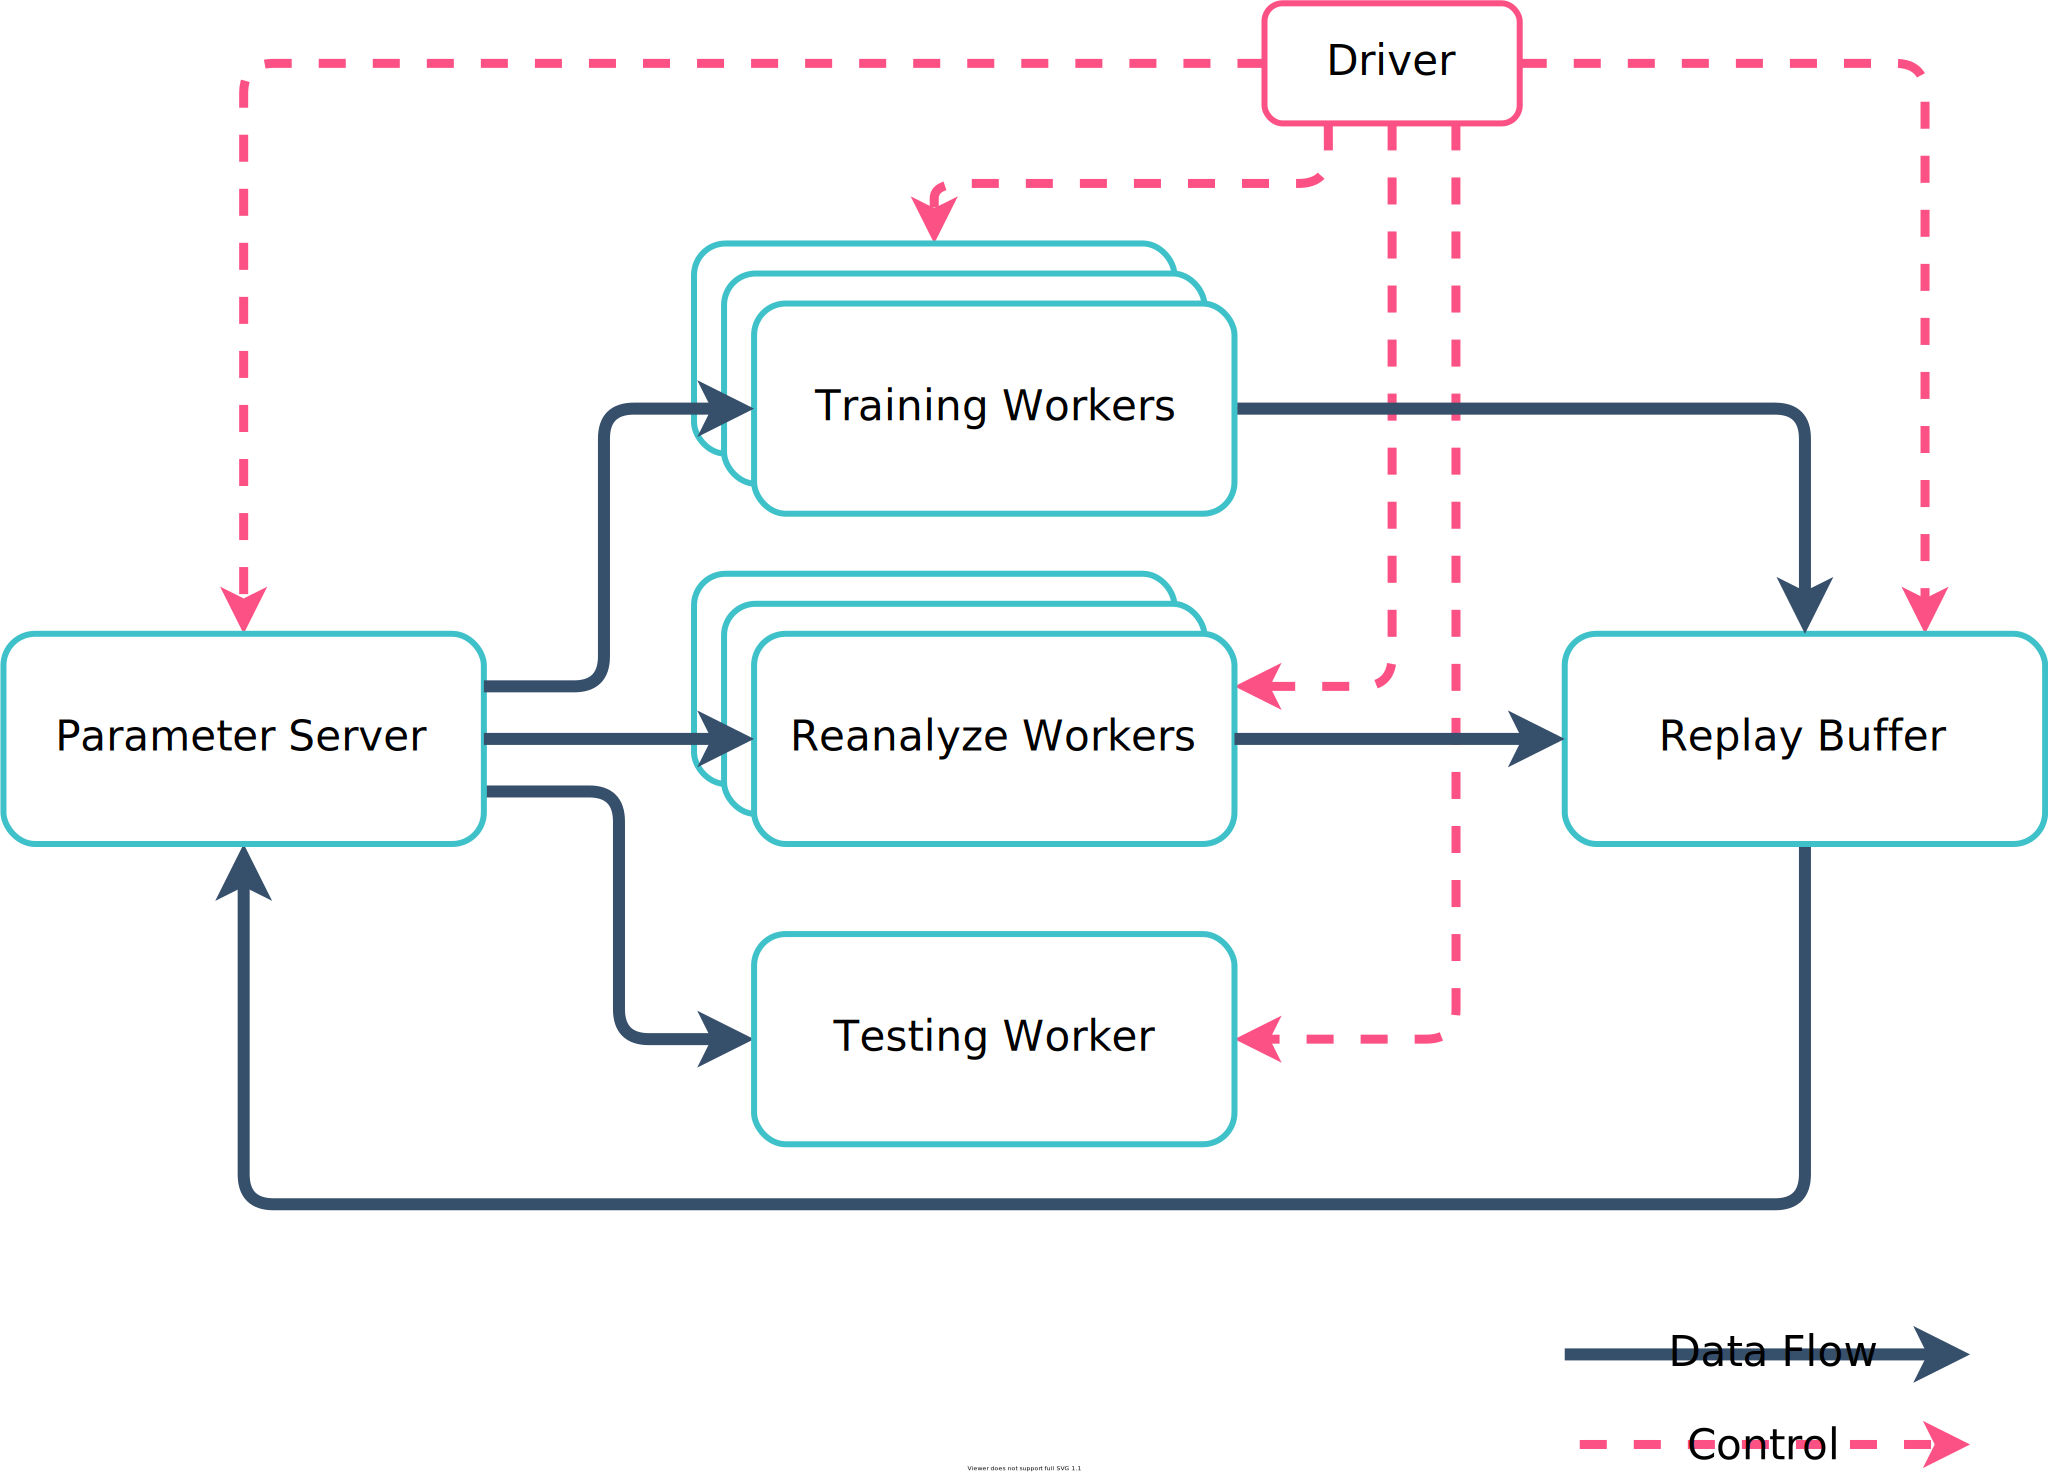
\includegraphics[width=\textwidth]{assets/moozi_architecture.png}
    \caption[]{MooZi Architecture}
    \label{fig:moozi_architecture}
\end{figure}

\subsubsection{Driver}
% MooZi adopts the \textbf{centralized control} design paradigm.
In a distributed system with centralized control, a single process is responsible for operating all other processes.
This central process is called the \textbf{driver}.
Other processes are either \textbf{tasks} or \textbf{actors}.
\textbf{Tasks} are stateless functions that takes inputs and return outputs.
\textbf{Actors} are statefull objects that group several methods that take inputs and return outputs.
In RL literature, \textbf{actor} is also a commonly used term to describe the process that stores a policy and interacts with an environment.
Even though MooZi does not adopt the concept of a RL actor, we will use the term \textbf{ray task} and \textbf{ray actor} to avoid confusion.
In contrast to distributed systems with distributed control, ray tasks and ray actors are reactive and do not have busy loops.
The driver decides when a ray task or ray actor is activated and what data should be used as inputs and where the outputs should go.
In other words, the driver process orchestrates the data and control flow of the entire system, and ray tasks and ray actors merely response to instructions.

\subsubsection{Environment Adaptors}
Environment adaptors unify environments defined in different libraries into a unified interface.
In the software engineering nomenclature, environment adaptors follow the adaptor design pattern \cite{AdapterPattern__2022}.

More specifically, in our project we implement environment adaptors for three types of environments that are commonly used in RL research:
(1) OpenAI Gym (2) OpenSpiel (3) MinAtar.
The adaptors convert the inputs and outputs of these environments into forms that GII accepts.

% Let's compare the libraries mentioned above with the agent-environment interface.
% In the agent-environment interface, the input to the environment is always a single action.
% Some of OpenSpiel's environments 

% return dict(
%     obs=timestep.observation,
%     is_first=timestep.first(),
%     is_last=timestep.last(),
%     to_play=0,
%     reward=reward,
%     legal_actions_mask=legal_actions_mask,
% )

The adaptors have the same signature as follows:
\begin{itemize}
    \item Inputs
          \subitem \textbf{is\_first}: A boolean signals the episode start.
          \subitem \textbf{is\_last}: A boolean signals the episode end.
          \subitem \textbf{action}: An integer indiates the last action taken by the agent.
          The valid range of the action is $\left[0, \text{number\_of\_available\_actions}\right)$.
    \item Outputs
          \subitem \textbf{obs}:
          An N-dimensional array that represents the observation of the current timestep.
          \subitem \textbf{is\_first}: A boolean signals the episode start.
          \subitem \textbf{is\_last}: A boolean signals the episode end.
          \subitem \textbf{to\_play}: An integer indicates the next player to take a move.
          \subitem \textbf{reward}: A float indicates the reward of taking the given action.
          \subitem \textbf{legal\_actions\_mask}: A bit mask of legal action indicies.
\end{itemize}

\subsubsection{Rollout Workers}
A \textbf{rollout worker} is a ray actor that:
\begin{itemize}
    \item stores a collection of universes, including tapes and laws in the universes
    \item stores a copy of the neural network specification
    \item stores a copy of the neural network parameters
    \item optionally stores batching layers that enable efficient computation
\end{itemize}

A rollout worker does not inherently serve a specific purpose in the system and its behavior is mostly determined by the list of laws created with the universes.

There are three main patterns of rollout workers used in MooZi:
\textbf{interaction training rollout worker},
\textbf{interaction testing rollout worker},
and \textbf{reanalyze rollout worker}.

\subsubsection{Replay Buffer}
The replay buffer:
\begin{itemize}
    \item stores trajectories generated by the rollout workers
    \item processes the trajectories into training targets
    \item stores processed training targets
    \item computes and updates priorities of training targets
    \item responsible for sampling and fetching batches of training targets
\end{itemize}

\subsubsection{Parameter Optimizer}
The parameter optimizer:
\begin{itemize}
    \item stores a copy of the neural network specification
    \item stores the latest copy of neural network parameters
    \item stores the loss function
    \item stores the training state
    \item computes forward and backward passes and updates the parameters
\end{itemize}

\subsubsection{Distributed Training}

\begin{python}
    for epoch in range(num_epochs):
    for w in workers_env + workers_test + workers_reanalyze:
    w.set_params_and_state(param_opt.get_params_and_state())

    while traj_futures:
    traj, traj_futures = ray.wait(traj_futures)
    traj = traj[0]
    replay_buffer.add_trajs(traj)

    if epoch >= epoch_train_start:
    train_batch = replay_buffer.get_train_targets_batch(
    big_batch_size
    )
    param_opt.update(train_batch, batch_size)

    env_trajs = [w.run(num_ticks_per_epoch) for w in workers_env]
    reanalyze_trajs = [w.run() for w in workers_reanalyze]
    traj_futures = env_trajs + reanalyze_trajs

    if epoch % test_interval == 0:
    test_result = workers_test[0].run(120)

    for w in workers_reanalyze:
    reanalyze_input = replay_buffer.get_train_targets_batch(
    num_trajs_per_reanalyze_universe
    * num_universes_per_reanalyze_worker
    )
    w.set_inputs(reanalyze_input)

\end{python}

\note{explain driver pseudo-code}

\subsubsection{Monte-Carlo Tree Search}
%     - asynchronous
%     - batching layer

\subsubsection{Logging and Visualization}


\section{Experiments}
\note{(20 pages)}

\section{Conclusion}
\note{(3 pages)}
\subsection{Future Work}
\note{(1 page)}

\printbibliography

\end{document}

% \subsection*{Artificial Intelligence}

% % Artificial Intelligence (AI) is a branch of computer science that emphasizes the use of computer algorithms to solve problems likes humans.
% To define the goals and methods of Artificial Intelligence (AI), we first need to define what is \textit{intelligence}.
% Though there is no consensus on the exact definition of intelligence, here we adopt the definition by John McCarthy:
% \begin{quote}
%     Intelligence is the computational part of the ability to achieve goals in the world.
% \end{quote}
% The goal of AI is to develop computer algorithms that can solve problems and achieve goals in complex environments.
% A diverse range of methods are designed as AI algorithms since the term has been coined.
% \note{A simple list of AI algorithms, such as A*, symbolic}


% \subsection*{Game Artificial Intelligence}
% Perfect vs in-Perfect information
% \subsection*{Planning}
% lookahead search: A*, DFS, BFS

% \subsection*{Distributed System for AI}
% IMPALA, SEED
